% !TEX root = tesis.tex

\chapter{Desarrollo de nueva electrónica para el SciCRT}
\chaptermark{Nueva electrónica}
\label{chap:tres}

Las necesidades del SciCRT operando en Sierra Negra no se acoplan directamente a los objetivos específicos de los experimentos K2K y SciBooNE, por lo que una de nuestras metas dentro de la colaboración ha sido el desarrollo de electrónica de alta velocidad de transferencia, bajo costo y consumo de potencia. Sumado a esto hemos decido seguir principios similares a los del desarrollo de software libre para evitar el \emph{vendor lock-in}. No obstante, encontrar una solución que cumpla de forma simultánea todos estos requerimientos resulta muy complejo. En este capítulo abordaré detalladamente el desarrollo del sistema de adquisición de datos, dando particular énfasis a su motivación científica. En este sentido el primero trataremos la velocidad de transferencia.

El primer paso en la dirección elegida fue desarrollar BE utilizando \emph{SiTCP} (procesador embebido programable desarrollado para experimentos de física de altas energías \cite{uchida08}) y la instalamos en uno de los SB que componen las capas de neutrones del telescopio \cite{ysasai17}. Gracias al uso de esta tecnología logramos alcanzar una tasa de transferencia de datos \num{10} veces mayor a la que teníamos con el bus VME. En la siguiente sección presentaré un estudio mediante simulación MC para evaluar el desempeño del SciCRT utilizando la electrónica de alta velocidad. Este análisis tiene también por objetivo mostrar la motivación detrás del requerimiento en la velocidad de transferencia. Hago notar que estudios similares se encuentran en: \cite{ynagai14,ysasai17}. El resultado original contenido en esta tesis lo presenté en la Conferencia internacional de Rayos Cósmicos en \emph{Busan}, Corea del Sur \cite{manzorena171}.

\section{Desempeño del SciCRT ante un evento de neutrones solares}

Evaluaremos la respuesta del SciCRT a un evento de neutrones solares mediante simulación MC, comparando el resultado con los datos obtenidos por el TNS instalado en Sierra Negra durante la ráfaga del \num{7} de Septiembre de \num{2005} \cite{sako06}. Este evento fue detectado por el TNS con una significacia de $17\sigma$ en el canal de partículas neutras con energías mayores a $>\SI{30}{\mega\electronvolt}$. El pico de la emisión de rayos \emph{X} duros (satélite Integral) fue a las 17:36:40 UT.

Si tomamos el flujo de neutrones solares para este evento, podemos estimar la significancia de las señales detectadas por el SciCRT en un evento similar. Para nuestra estimación consideraremos como parámetros de entrada \cite{ynagai14}: un espectro de energía de los neutrones en el Sol de acuerdo a una ley de potencias
$\num{6.1e27}\left(E/\si{\mega\electronvolt}\right)^{-3.8}\si{\per\mega\electronvolt\per\steradian}$, neutrones emitidos de manera impulsiva en el Sol y un ángulo cenital de \ang{17.5}. La propagación de los neutrones solares en la atmósfera terrestre se simula usando el modelo de Shibata.

\begin{figure}
\centering
  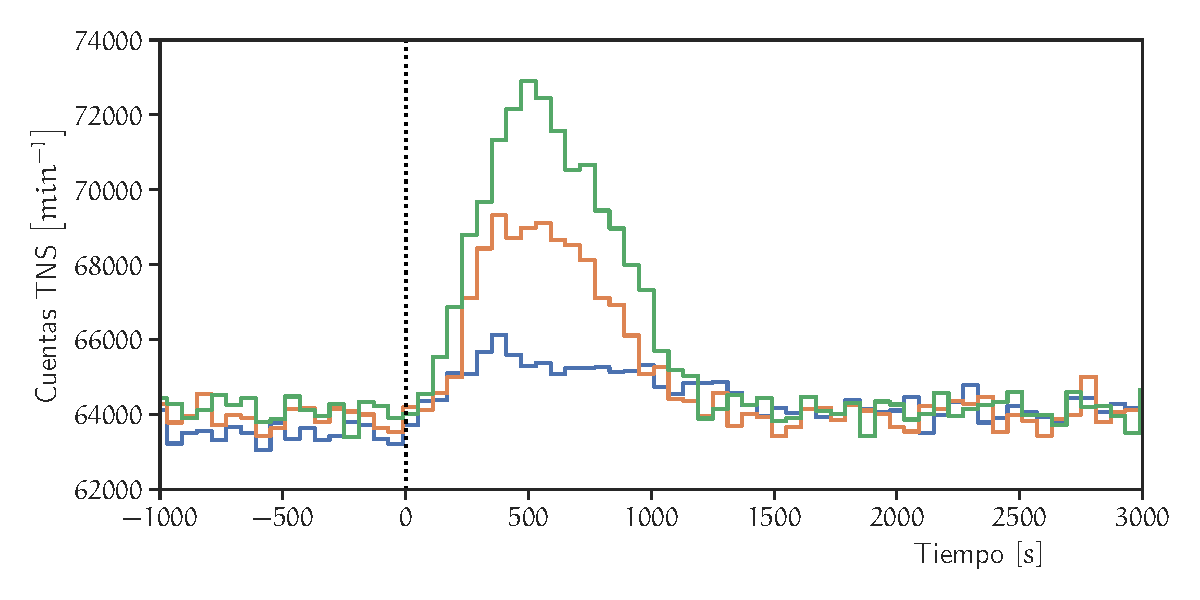
\includegraphics[width=\textwidth]{scicrt-sim.pdf}
  \caption{Simulación de los perfiles temporales del SciCRT asumiendo un flujo de neutrones solares similar al del evento del \num{7} de Septiembre de \num{2005}. La curva azul muestra los datos obtenidos por el TNS, la línea naranja es el perfil temporal del SciCRT usando la electrónica original. La línea roja muestra el caso cuando instalamos la electrónica de alta velocidad. Los datos están normalizados al nivel de fondo del TNS. La línea punteada indica el instante en que la intensidad de rayos X duros alcanzó su máximo valor.}
  \label{fig:solar-sim}
\end{figure}

Los resultados de nuestro cálculo se muestran en la figura \ref{fig:solar-sim}. Es importante aclarar que para esta estimación tomamos en cuenta dos situaciones; una con la electrónica original y otra con la electrónica de alta velocidad, ambas instaladas en $4/8$ del detector. La línea punteada en \SI{0}{\second} indica el instante en que la intensidad de rayos \emph{X} duros alcanzó su valor máximo. En la figura la linea azul representa los datos del TNS de partículas neutras con $E_{k}>\SI{30}{\mega\electronvolt}$. El perfil temporal de las cuentas del SciCRT con la electrónica original (línea naranja) muestra una significacia de $39\sigma$, lo que se traduce en una sensibilidad \num{2.3} veces mayor a la del TNS durante el mismo evento. Sin embargo, al tomar en cuenta el caso de la nuevo DAQ (línea verde), el incremento es de $59\sigma$, es decir, \num{3.5} veces mayor sensibilidad.

Con respecto a los datos de energía depositada (considerando el uso de electrónica de alta velocidad) el incremento también notable puesto que se tiene una sensibilidad \num{3} veces mayor, con la ventaja extra de que podemos estimar el espectro de los neutrones con una excelente resolución \cite{ysasai17}.

A pesar de este resultado positivo, la sensibilidad del detector es directamente función del volumen activo del telescopio. Para justificar este punto, la figura \ref{fig:eficiencia-electronica} muestra la eficiencia de detección de neutrones en función del número de SB instalados y la energía incidente. La línea azul representa el caso para un SB, la línea naranja dos SB y la verde cuatro. De la figura es posible concluir que la eficiencia de detección de neutrones incrementa principalmente en la zona de bajas energías ($<$\SI{100}{\mega\electronvolt}). Este resultado concuerda con lo expuesto en \cite{nagaiphd}, el cual reporta una eficiencia del \SI{30}{\percent} para neutrones de \SI{50}{\mega\electronvolt} considerando la instalación completa del SciCRT. En el caso de los neutrones de mayor energía, aunque la eficiencia de detección no incrementa de forma significativa con el número de SB instalados, las capacidades para estudiar el espectro de energía y la distribución angular si son mejoradas.

Adicionalmente, dada la operación del telescopio en alta montaña, la operación sostenible a largo plazo requiere de la producción de electrónica de bajo costo y potencia de consumo, ya que las condiciones ambientales reducen la vida útil de los componentes, además de dificultar la disipación de calor. Tomando en cuenta todo lo anterior y considerando que solo $3/8$ de la electrónica total necesaria para la instalación está disponible en estos momentos, el desarrollo de nuevas unidades de \emph{front end} se vuelve una prioridad de nuestro experimento.

\begin{figure}
        \centering
        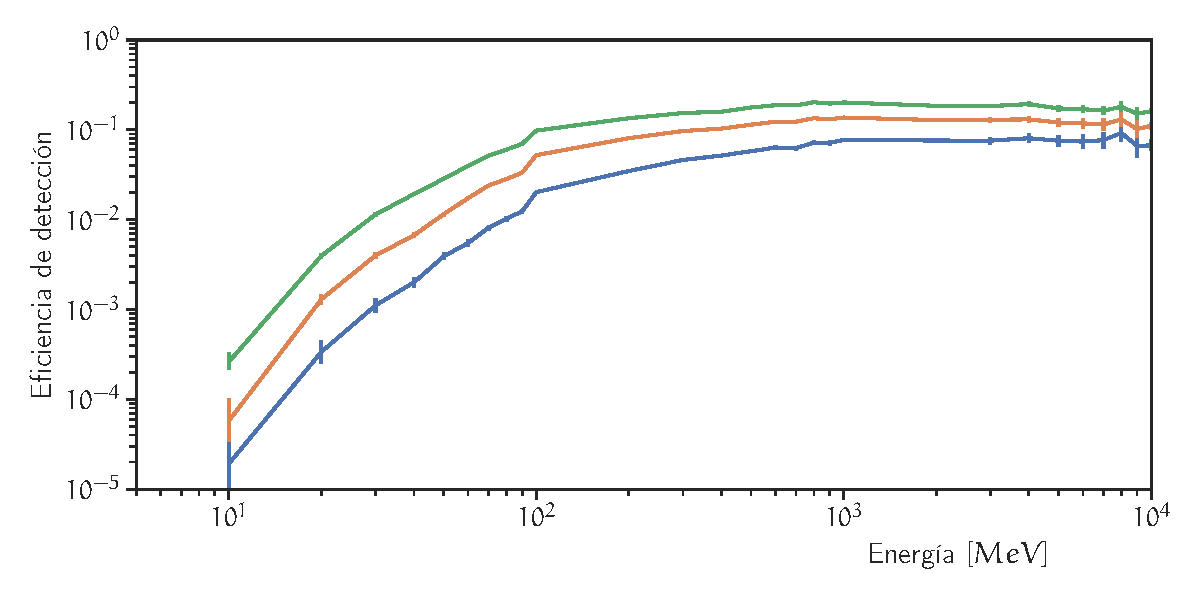
\includegraphics[width=\textwidth]{electronics-deff.pdf}
        \caption{Eficiencia de detección de neutrones en función de SB instalados. La gráfica azul representa la eficiencia con un SB, la gráfica naranja es con dos SB y la verde con cuatro SB.}
        \label{fig:eficiencia-electronica}
\end{figure}

\section{La técnica de \emph{Time over threshold}}
\label{sec:time-over}

Como mencioné en el capitulo \ref{chap:dos}, cuando una partícula energética entra en el volumen activo de un detector, ésta pierde su energía interaccionando con el medio. Considerando una partícula con carga eléctrica, la energía depositada se puede estimar midiendo las pérdidas por ionización; el número de iones generados al atravesar el detector. En el caso de un material centellador la medida de la pérdida por ionización es el número de fotones.

De esta forma, el cálculo de la carga depositada $Q$ en el detector se puede realizar integrando la señal de corriente:

\begin{equation}
\label{equ:charge}
Q=\int_{0}^{T_{max}} i_{pmt}\left(t\right)\mathrm{d}t
\end{equation}

de donde $T_{max}$ es el tiempo de corte, el cual se debe escoger lo más grande posible para garantizar que la integración incluya la mayor cantidad de fotoelectrones\footnote{Idealmente este tiempo debe ser infinito, sin embargo esto lleva a la saturación de la electrónica.}. Luego entonces una método sencillo para procesar este tipo de información consiste en integrar los pulsos para posteriormente digitalizarlos. Esto constituye la base de las técnicas convencionales de procesamiento de pulsos ampliamente utilizadas en electrónica nuclear.

Con la llegada de sistemas de detección de radiación de gran escala (sistemas de miles de canales o más), los métodos basados en digitalización de pulsos se implementan en circuitos de aplicación específica (ASIC); lo cual permite una excelente resolución de energía, bajo consumo de potencia y tamaño reducido; a expensas de altos costos de producción y desarrollo.

Por esta razón el desarrollo de la instrumentación del SciCRT requiere de un método de estimación de energía que se adapte a las necesidades de nuestro experimento.

Una alternativa es el uso de la técnica de \emph{Time over threshold} (TOT), la cual permite una arquitectura simplificada a cambio de un pérdida en la linealidad y compresión en el rango dinámico \cite{fujiwara10}. En este método una señal digital variante en el tiempo TOT codifica la información de la amplitud del pulso, a partir del tiempo que dura el pulso analógico por encima de un umbral predefinido. Posteriormente se necesita convertir la información temporal a valores digitales usando un \emph{time digital converter} (TDC).

Para aplicar este método el primer paso será encontrar una relación entre $Q$ y TOT, lo cual se puede hacer resolviendo un sistema de ecuaciones no lineales. Si consideramos $s\left(t\right)$ la señal con la información de la carga y $v\left(t\right)$ la función que describe al umbral, el sistema de ecuaciones se puede escribir como:

\begin{equation}
\label{equ:tot-equ}
\begin{aligned}
\left. s\left(t\right)\right|_{t=ti} &= \left. v\left(t\right)\right|_{t=ti}\\
\left. s\left(t\right)\right|_{t=tf} &= \left. v\left(t\right)\right|_{t=tf}
\end{aligned}
\end{equation}

donde $t_{i}$ y $t_{f}$ representan los puntos en que la señal rebasa el umbral. Es importante notar que $TOT=t_{f}-t_{i}$. Resolviendo este sistema para el caso particular de un pulso de centelleo del tipo exponencial obtenemos:

\begin{equation}
\begin{aligned}
TOT &= -\ln\left(\dfrac{V_{th}}{s_{0}}\right)^{\tau_{d}}\\
 &= \tau_{d} \ln\left(s_{0}\right)-K
\end{aligned}
\end{equation}

de donde $s_{0}$ representa la distribución de amplitudes del pulso (energía depositada), $\tau_{d}$ la constante del centellador y $V_{th}$ el umbral para l conversión. Con este modelo simplificado podemos observar que la relación entre la carga y el TOT no es lineal. Para verificar este comportamiento realizaremos una simulación de primeros principios tomando las características similares a las de las señales del SciCRT. Primero consideramos que $s_{0}$ es una variable aleatoria distribuida normalmente $X\ \sim\ \mathcal{N}\left(\mu,\,\sigma^2\right)$, con media $\mu$ y desviación estándar $\sigma$.

El resultado de la simulación se presenta en la figura \ref{fig:tot-model}. Los paneles superior en inferior izquierdo muestran los pulsos simulados y la distribución de amplitudes, respectivamente. Por otro lado, el panel superior derecho en la figura muestra la relación que existe entre $Q$ y TOT para las señales descritas. El panel inferior derecho muestra la distribución de los valores de TOT. Idealmente esta distribución debe ser la misma que la del panel izquierdo, sin embargo, debido a la relación no lineal entre $Q$ y TOT, observamos una distorsión en el área de baja energía; lo cual limita el rango dinámico del método.

Esta limitante del método nos obliga a ser cuidadosos en la elección de parámetros de diseño de nuestro sistema, ya que sin un análisis detallado se corre el riesgo perder resolución en energía. Como expondré más adelante, esto me motivo a realizar un estudio mediante simulación buscando optimizar los parámetros de diseño.

\begin{figure}
        \centering
        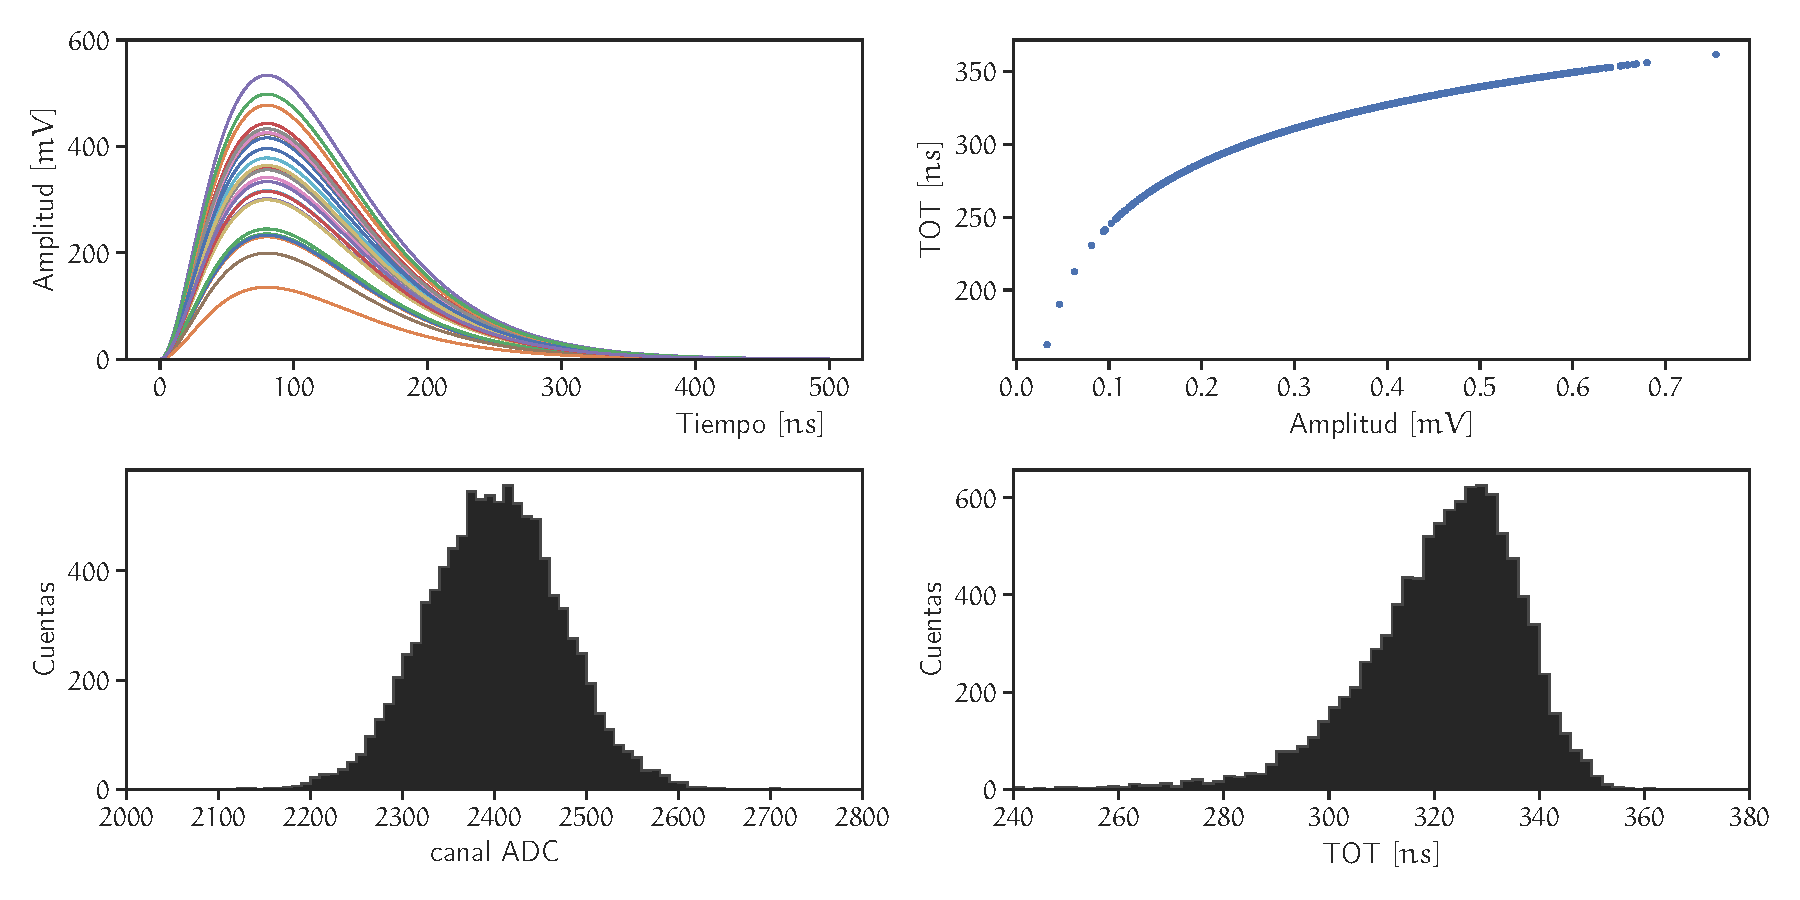
\includegraphics[width=\textwidth]{TOT-model.pdf}
        \caption{Modelo de primeros principios de conversión Carga-TOT.}
        \label{fig:tot-model}
\end{figure}

Aunado a este problema, es importante establecer que la señal a la salida del detector no es útil para extraer la información de la carga depositada del evento de radiación ya que es de corta duración. Debido a esto, el primer paso antes de poder procesar la señal de radiación es acondicionar la señal para que tenga una mayor duración y una amplitud máxima definida. El efecto de incrementar la duración de la señal, mejora la razón señal a ruido, mientras que la amplitud definida permite la lectura correcta de la información de la carga. Esto lleva a que el proceso de optimización requiera el estudio de los diversos elementos que comprenden el sistema.

El diagrama esquemático del sistema TOT propuesto se muestra en el panel superior de la figura \ref{fig:nfeb-prot}. El uso de un dispositivo programable como el FPGA (field programmable gate array) permite la integración de la mayoría de las funciones requeridas por el sistema de procesamiento de pulsos, incluido SiTCP que nos permite hacer la transferencia de datos rápida. La principal ventaja de esta integración es que permite reducir el costo de desarrollo y producción.

La parte analógica del sistema está compuesta por un ciruito preamplificador y un formador. El preamplificador tiene como función convertir la señal de corriente del fotomultiplicador en una señal de voltaje, llevando a cabo en el proceso la integración de la señal de corriente. El formador es un filtro pasa banda, en el cual además de amplificar la señal de la etapa anterior, también define las características temporales (tiempos de subida, bajada y duración) de la señal del detector. Considerando que la mayor parte del sistema es digital, y que ésta se puede implementar en un sólo dispositivo: el tamaño de la tarjeta queda principalmente definido por el número de componentes utilizados para construir la sección de procesamiento analógico. Por esta razón el diseño de este bloque tiene como restricción encontrar un solución que utilice una cantidad de elementos pequeña. Una arquitectura básica para este bloque se muestra en el panel inferior de la figura \ref{fig:nfeb-prot}, la cual se describirá más adelante.

A continuación presentó el diseño del sistema TDC usando la técnica de sobremuestreo, el cual tiene el fin de alcanzar una buena resolución temporal y un bajo uso de los recursos del circuito programable.

\begin{figure}
        \centering
        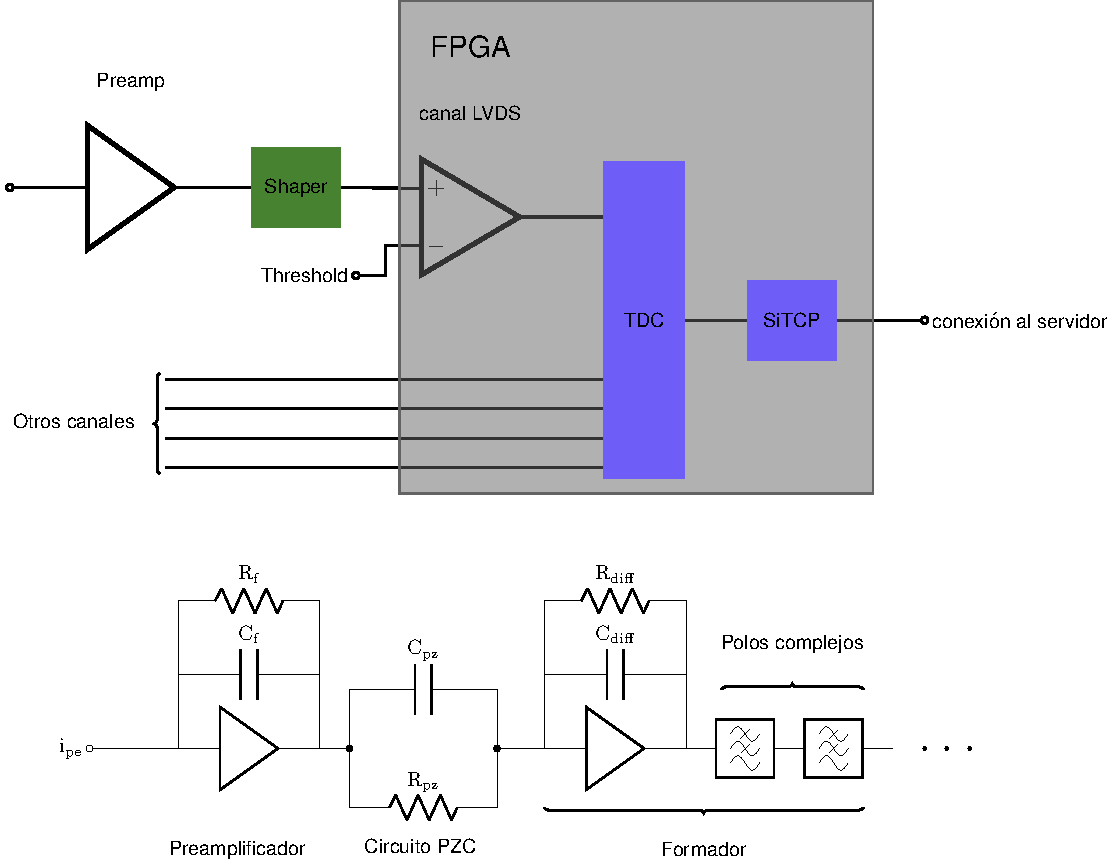
\includegraphics[width=\textwidth]{nfeb-prot.pdf}
        \caption{Diagrama esquemático de la nueva electrónica del SciCRT (panel superior). Circuito de amplicación y formación (panel inferior).}
        \label{fig:nfeb-prot}
\end{figure}

\section{Diseño de un \emph{Time digital converter} con sobremuestreo}

La arquitectura básica de un TDC está compuesta por un contador digital y un circuito detector de flancos (detección de inicio y fin de la señal a medir). A pesar de que este sistema puede tener un amplio rango dinámico de medición, la principal desventaja es la resolución temporal; ya que depende directamente de la frecuencia de reloj. Debido a esto resulta complejo en práctica alcanzar resoluciones temporales menores a \SI{10}{\nano\second} con esta arquitectura.

Un técnica empleada para superar esta limitación es el sobremuestreo \cite{spencer06,balla14}, cuyo principio de funcionamiento se ilustra en la figura \ref{fig:tdc-diagram}. Un TDC con sobremuestreo se compone de dos unidades: un contador grueso y un interpolador. El contador opera a una frecuencia $F_{0}=1/T_{0}$, con él se obtiene una medida \emph{entera} del número de ciclos de reloj que dura la señal a medir (en nuestro caso TOT). El interpolador se encarga de medir la parte fraccionaria del ciclo de reloj, utilizando para esto $N$ copias de la señal de reloj. Como se observa en la parte derecha de la figura \ref{fig:tdc-diagram}, las copias están retrasadas una respecto a la otra por un factor de $T_{0}/N$.  La lógica dentro del sistema interpolador se encarga de determinar cuál de las copias de la señal de reloj fue la primera en observar la transición de la señal a medir y fija un valor binario. El resultado de la medición del intervalo de tiempo es la suma la parte entera y la fraccionaria.

\begin{figure}
        \centering
        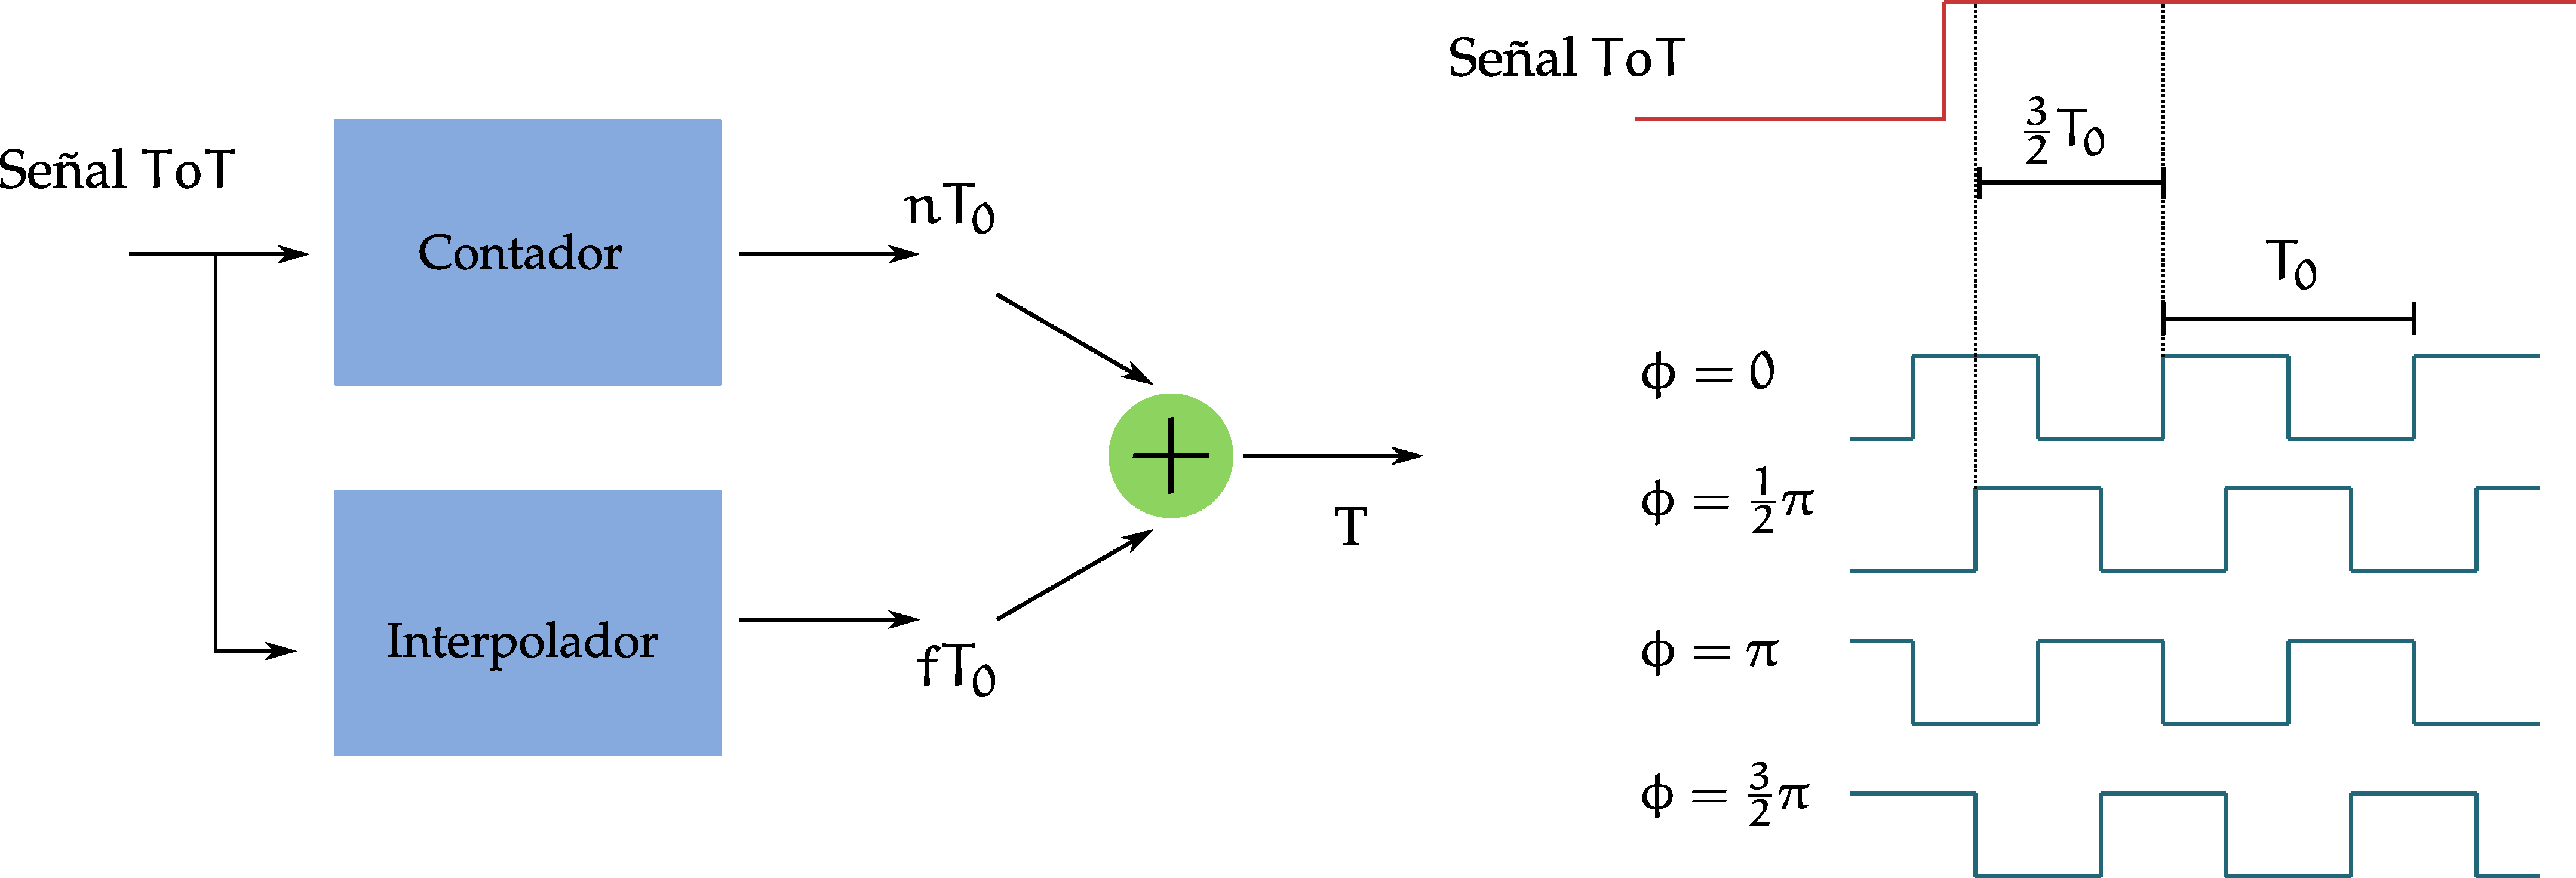
\includegraphics[width=\textwidth]{tdc-diagram.pdf}
        \caption{Arquitectura básica del sistema TDC por interpolación (panel izquierdo). Diagrama de tiempo y principio de operación del sistema TDC por interpolación.}
        \label{fig:tdc-diagram}
\end{figure}

Procedí a describir un módulo TDC en un FPGA usando un factor de sobremuestreo de \num{8}, con lo que pude obtener resoluciones temporales de \SI{0.5}{\nano\second} a \SI{2.5}{\nano\second}. En este modulo también incluí la transferencia de datos usando SiTCP. La precisión del convertidor fue medida usando una señal a la entrada de \SI{7.71}{\nano\second} de duración y una frecuencia de repetición de \SI{1}{\kilo\hertz}. En total obtuve una muestra de \num{1e5} eventos. La frecuencia de la señal a medir nos sirve para caracterizar el \emph{tiempo muerto} del sistema de adquisición y determinar si la velocidad de transmisión entre éste y la PC es suficiente para procesar la información obtenida del detector. Los resultados de la prueba se muestran en el histograma de la figura \ref{fig:tdc-lvds}.

\begin{figure}
        \centering
        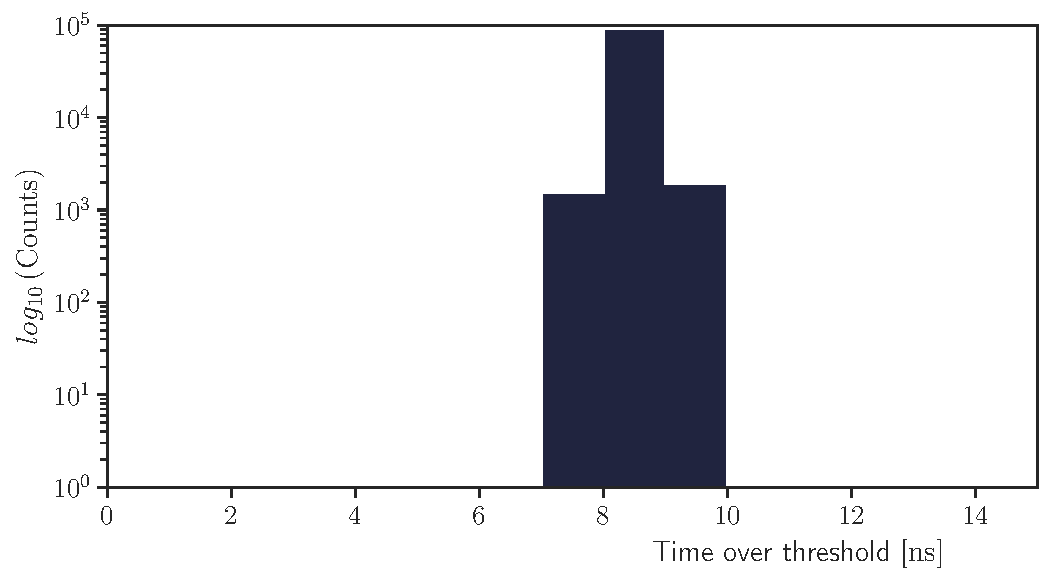
\includegraphics[width=\textwidth]{tot-lvds.pdf}
        \caption{Precisión del circuito TDC con una resolución de \SI{1}{\nano\second}. La prueba se realizó con una señal de \SI{7.71}{\nano\second} de duración y una frecuencia de repetición de \SI{1}{\kilo\hertz}.}
        \label{fig:tdc-lvds}
\end{figure}

Al analizar los resultados de la figura, podemos concluir que son satisfactorios; ya que al utilizar un TDC con resolución de \SI{1}{\nano\second}, el \emph{bin} más cercano a la duración que deseamos medir es \SI{8}{\nano\second} y más del \SI{96}{\percent} de los eventos se encuentran en ese \emph{bin}. Solo el \SI{4}{\percent} de los eventos tienen una error producido debido a errores de sincronía del interpolador (los eventos entre \SI{7}{\nano\second} y \SI{9}{\nano\second}). Es importante mencionar que estos errores están directamente relacionados con el \emph{jitter} (fluctuaciones aleatorias en las fases) en la señal a medir y/o la señal de reloj.

\section{Diseño y optimización de la electrónica}

Para diseñar el circuito preamplificador utilizamos una configuración de \emph{charge sensitive amplifier}, con un capacitor $C_{f}$ y una resistencia $R_{f}$ en el lazo de realimentación. De esta forma, tres parámetros son necesarios para la especificación de este sistema: los valores de $C_{f}$, $R_{f}$ y el ancho de banda mínimo del amplificador. La razón $S/N$ del preamplificador es sensible a estos parámetros, sin embargo considerando que nuestro fotosensor es un MAPMT, el número de fotoelectrones en la señal es el factor dominante. Con respecto a este punto, suponiendo la señal producida un muon que interacciona con una de las barras del SciCRT en el extremo más alejado del sensor (ver \ref{chap:dos}), sabemos que en promedio llegan al sensor \SI{10}{pe}. Esto se traduce en una señal de amplitud considerable (\SI{200}{\milli\volt}), lo cual nos permite concluir que el efecto de $C_{f}$ y $R_{f}$ en $S/N$ es despreciable.

Las características del pulso después del procesamiento analógico (duración y amplitud) son afectadas directamente por el preamplificador, y debido a esto deben ser consideradas para la optimización del TDC. Un punto importante dentro de esto es la minimización del ruido de cuantización, lo cual puede alcanzarse utilizando de manera efectiva el rango dinámico del amplificador (buscando evitar la saturación) y el TDC. Para esto realizamos una simulación MC incluyendo la respuesta en frecuencia del preamplificador y el circuito formado (el cual se describe más adelante); variando el valor de $C_{f}$ en el rango de \num{10} a \SI{500}{\pico\farad}. De esta forma obtenemos la relación lineal entre el número de fotoelectrones en la pulso de entrada (\si{pe}) y la amplitud del pulso de salida. El valor de $R_{f}$ se selecciona en el rango de \num{1} a \SI{50}{\kilo\ohm} de forma que la constante de integración sea aproximadamente \SI{600}{\ns}.

La figura \ref{fig:phe-cal} muestra el resultado de este análisis para $C_ {f}=20,40$ y \SI{100}{\pico\farad}, lo cual resulta en tres estructuras lineales distintivas. Los colores en la figura representan valores diferentes $R_{f}$ mientras $C_{f}$ permanece constante. Las líneas horizontales en la figura indican dos diferentes voltajes de saturación: \SI{5}{\volt} y \SI{2.5}{\volt}, correspondientes a dos diferentes tipos de amplificadores. A partir de esto podemos concluir que la pendiente de las curvas en la figura (la ganancia de conversión) es principalmente controlada por $C_{f}$, mientras que es relativamente insensible a cambios de $R_{f}$. Considerando que el rango dinámico de la señal de muones de \num{1} a \SI{250}{pe} (como se mostró en el capítulo \ref{chap:dos}), el valor óptimo para $C_{f}$ está entre \SI{20}{\pico\farad} y \SI{40}{\pico\farad} para el caso de amplificadores con $V_{sat}=\SI{5}{\volt}$.

\begin{figure}
        \centering
        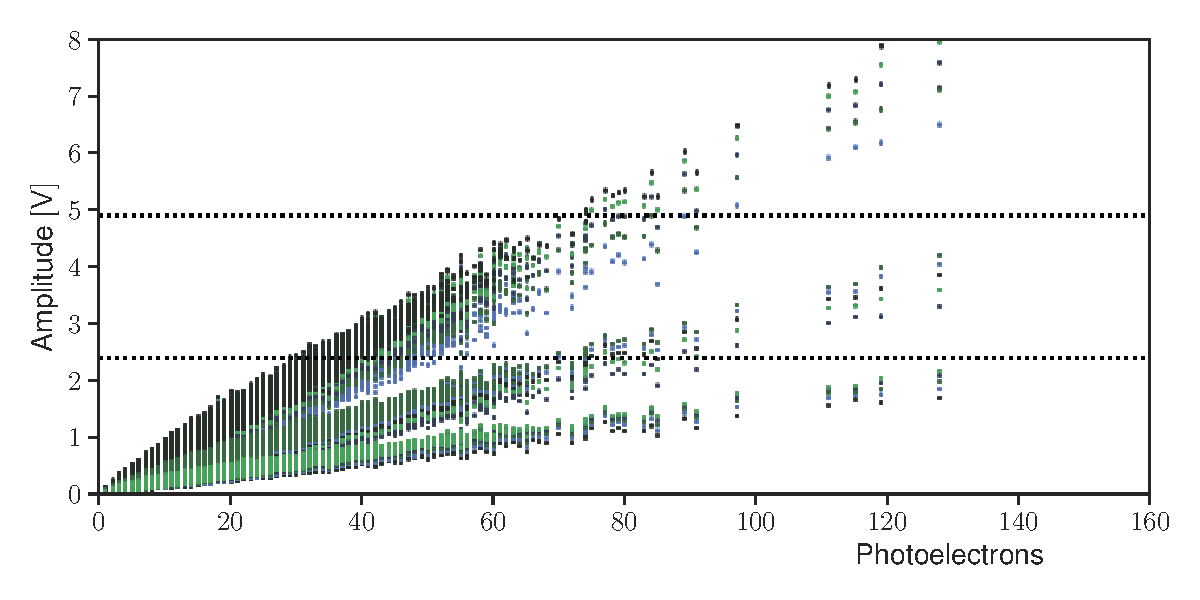
\includegraphics[width=\textwidth]{phe-cal.pdf}
        \caption{Respuesta del preamplificador en función de los elementos de realimentación. La ganancia de conversión (la pendiente de las estructuras lineales) es controlada principalmente por $C_{f}$. Los colores en la figura representan cambios en $R_{f}$ mientras $C_{f}$ se mantiene constante. Para más detalles ver el texto.}
        \label{fig:phe-cal}
\end{figure}

Lo siguiente es analizar la conversión de la señal analógica a una señal TOT. El análisis requiere que definamos el método de formación de las señales y las características del TDC. Es importante recordar que,  junto con el consumo de potencia del circuito, los parámetros del TDC sirven de restricción al problema de optimización ya que el uso eficiente del rango dinámico disminuye la distorsión por ruido de cuantización. Para el circuito formador utilicé un filtro Gaussiano ya que éste se desempeña satisfactoriamente en aplicaciones con altas tasas de cuentas \cite{ohkawa76}.

Haciendo un análisis similar al de la sección \ref{sec:time-over} usando una forma de pulso Gaussiana, podemos escribir la relación entre el número de fotoelectrones y el TOT de la siguiente forma:

\begin{equation}
\label{equ:tot-nphe}
T_{OT}^{2}=2\sigma^{2}\ln{k_{0} N_{phe}}-w_{th}
\end{equation}

en donde $N_{phe}$ es el número de fotoelectrones, $k_{0}$ es la ganancia de conversión del preamplificador, $\sigma$ es el tiempo de formación del cicuito y $w_{th}$ es una constante de calibración; dependiente del umbral usando para el TOT y $\sigma$. Usando la ecuación \ref{equ:tot-nphe} y considerando que $k_{0}$ fue determinada en el análisis anterior, las características de la señal del detector se pueden convertir de forma eficiente cambiando $\sigma$ y el umbral del sistema.

La simulación completa de la electrónica considera el preamplificador, circuito formador y conversión a digital usando el TDC. El rango y resolución del TDC se seleccionan a partir de los resultados de la simulación, considerando los casos en donde el rango de la señal del detector ocupa la mayor cantidad de \emph{bins}. A partir de esto determiné que una con una resolución de \SI{1}{\ns\per bin} y \SI{8}{bits \per muestra} es posible convertir la señal de manera efectiva. La figura \ref{fig:tot-sigma} muestra el resultado de la simulación usando la resolución óptima de TDC, para diferentes valores de $\sigma$ del formador ($\sigma=70,100$ y $\SI{125}{\ns}$). En cada panel de la figura la escala de colores representa un umbral distinto, desde azul (\SI{10}{\milli\volt}) claro hasta el verde claro (\SI{50}{\milli\volt}). Es evidente de la figura que el rango dinámico del convertidor se ocupa mejor con $\sigma=\SI{125}{\ns}$.

\begin{figure}
        \centering
        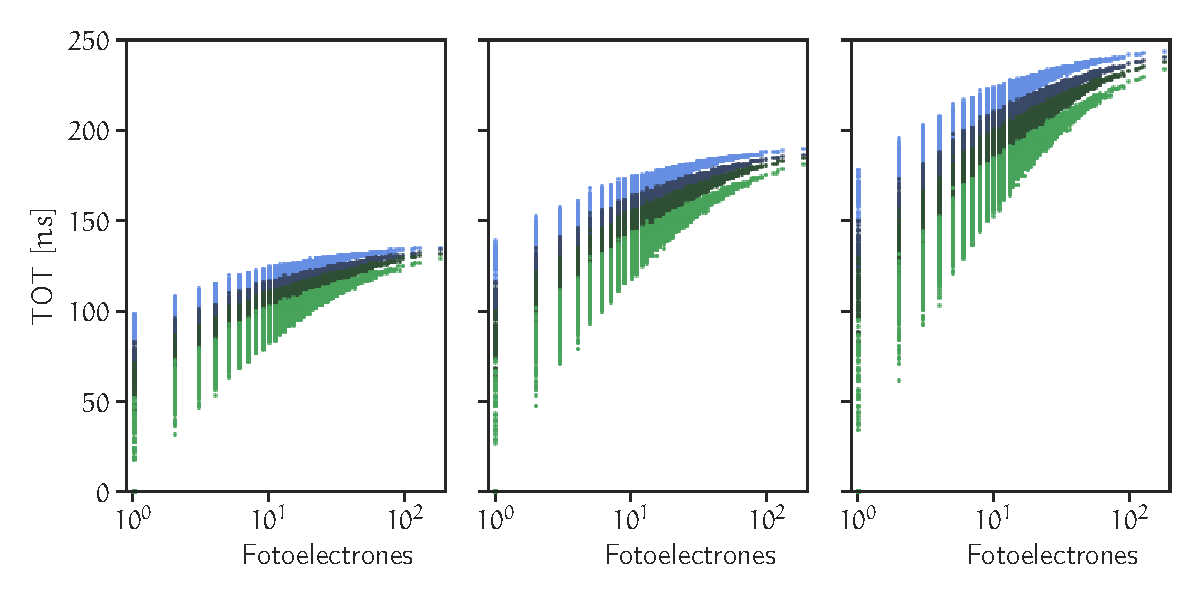
\includegraphics[width=\textwidth]{tot_d30par.pdf}
        \caption{Características del TOT para señales de muones simuladas usando formadores Gaussianos de diferente escala. El panel de la izquierda es con $\sigma=70$, el panel del centro corresponde a $\sigma=100$ y el panel de la derecha es $\sigma=125$. Los colores representan cambios en el umbral, desde \SI{10}{\milli\volt} (azul claro) a \SI{50}{\milli\volt} (verde claro).}
        \label{fig:tot-sigma}
\end{figure}

Con el objetivo de implementar el circuito formador usamos el método descrito en \cite{ohkawa76}, el cual es un método muy usado en el desarrollo de electrónica nuclear. Bajo este marco de referencia solo se necesitan dos parámetros para especificar el diseño: el orden del filtro $N$ y su topología. El orden del filtro mejora la respuesta temporal del circuito disminuyendo el efecto del \emph{pile-up}, con la desventaja de incrementar el consumo de potencia. Tras el análisis escogí un filtro de orden $N=3$ ya que ofrecía la mejor respuesta en términos de desempeño y consumo de potencia.

Para finalizar el análisis mediante simulación del diseño, estudié el posible efecto de dependencia entre el TOT y la distancia al MAPMT. Considerando que uno de los extremos de las barras está pintado para mejorar la eficiencia de recolección, es de esperarse un ensanchamiento en la estructura temporal de los pulsos a medida que la partícula cruza el centellador a distancias más cortas del fotosensor. La figura \ref{fig:tot-distance} muestra el resultado de simular \num{1e6} muones cruzando la barra centelladora a diferentes distancias del MAPMT. Como se esperaba, los pulsos generados cerca del sensor son más anchos que los generados en el otro extremo. No obstante, el efecto es muy pequeño; incapaz de producir alguna saturación en la electrónica. Queda la posibilidad de que relación lineal entra estas variables pueda ser útil en el futuro para corregir los datos registrados, en un análisis similar al hecho con la atenuación de la fibra.

\begin{figure}
        \centering
        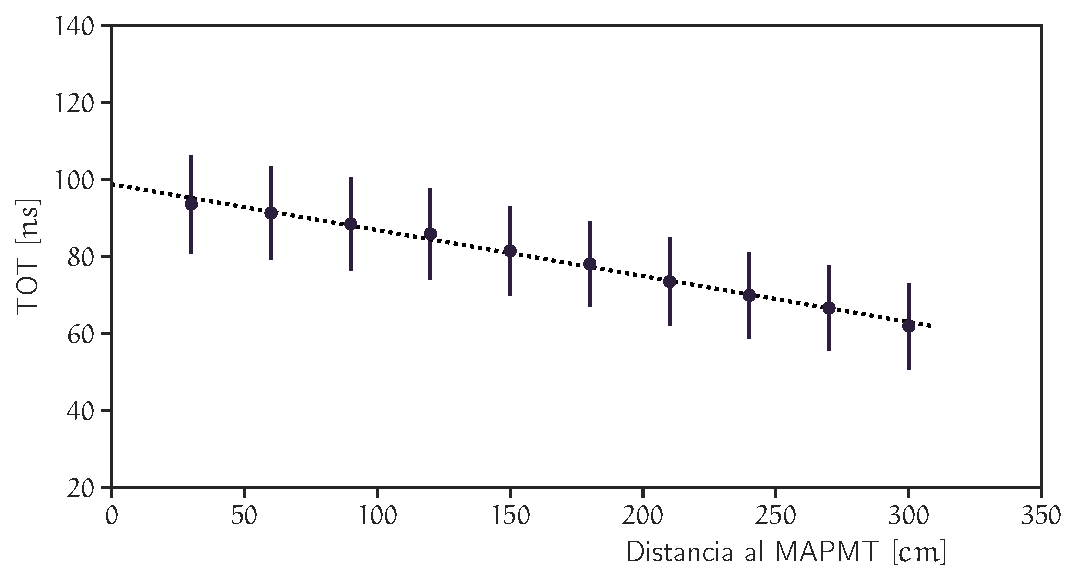
\includegraphics[width=\textwidth]{tot_distance.pdf}
        \caption{Valores promedio de TOT a diferentes distancias del MAPMT, incluyendo barras de error de $\pm\sigma$. La línea punteada representa el resultado del ajuste lineal.}
        \label{fig:tot-distance}
\end{figure}

El circuito final del preamplificador/formador se muestra en la \ref{fig:preamp-shaper}. La elección del modelo del amplificador operacional se hizo considerando el ancho de banda mínimo con vista a reducir el consumo de potencia. A partir de la simulación estimé que el circuito requiere un mínimo ancho de banda de \SI{200}{\mega\hertz}. Con esto seleccioné dos modelos de amplificadores, el ADA4891 y ADA4807, ambos de Analog Devices. Ambos circuitos tienen una respuesta en frecuencia similar, sin embargo difieren en consumo de potencia y precio.

Durante una estancia de investigación en el ISEE (Institute) de la Universidad de Nagoya, Japón, construí un prototipo de \num{16} canales de la electrónica FE. El prototipo utiliza el amplificador ADA4891 y fue probado con LED verde (pico de emisión \SI{505}{\nano\metre}). La parte digital del sistema la implementé usando una tarjeta Spartan \num{6} de Xilinx, la cual realiza las tareas de discriminación, TDC y transferencia de datos usando SiTCP. Para la interconexión del sistema fue además necesario desarrollar circuito capaz de distribuir la alimentación y señales de reloj del sistema utilizando la capa física del Ethernet. La figuras \ref{fig:neutron-pcb} y \ref{fig:complete-sys} muestran la tarjeta diseñada, así como el prototipo en operación.

\begin{figure}
        \centering
        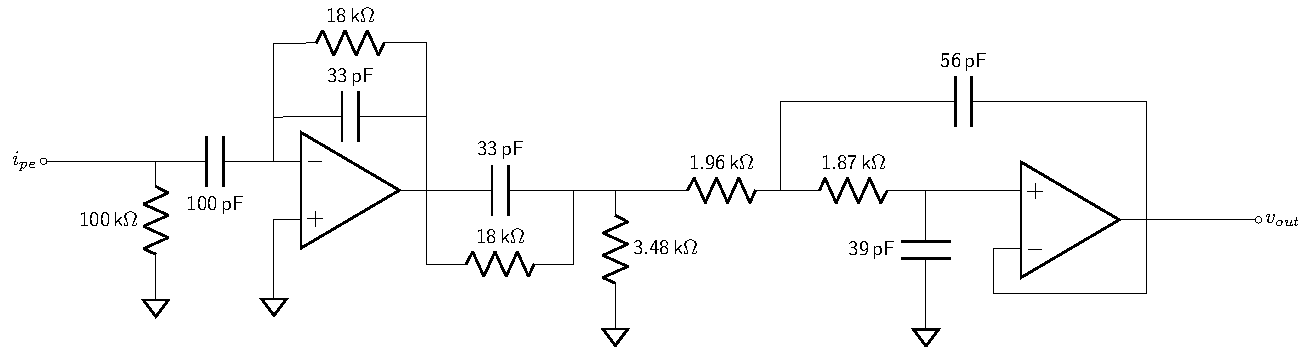
\includegraphics[width=\textwidth]{preamp-shaper-final.pdf}
        \caption{Diagrama esquemático del circuito preamplificador/formador. Para el análisis mediante la simulación MC consideramos dos modelos de amplificadores: ADA4891 y ADA4807.}
        \label{fig:preamp-shaper}
\end{figure}

\begin{figure}
  \centering
  \begin{subfigure}[b]{0.49\textwidth}
	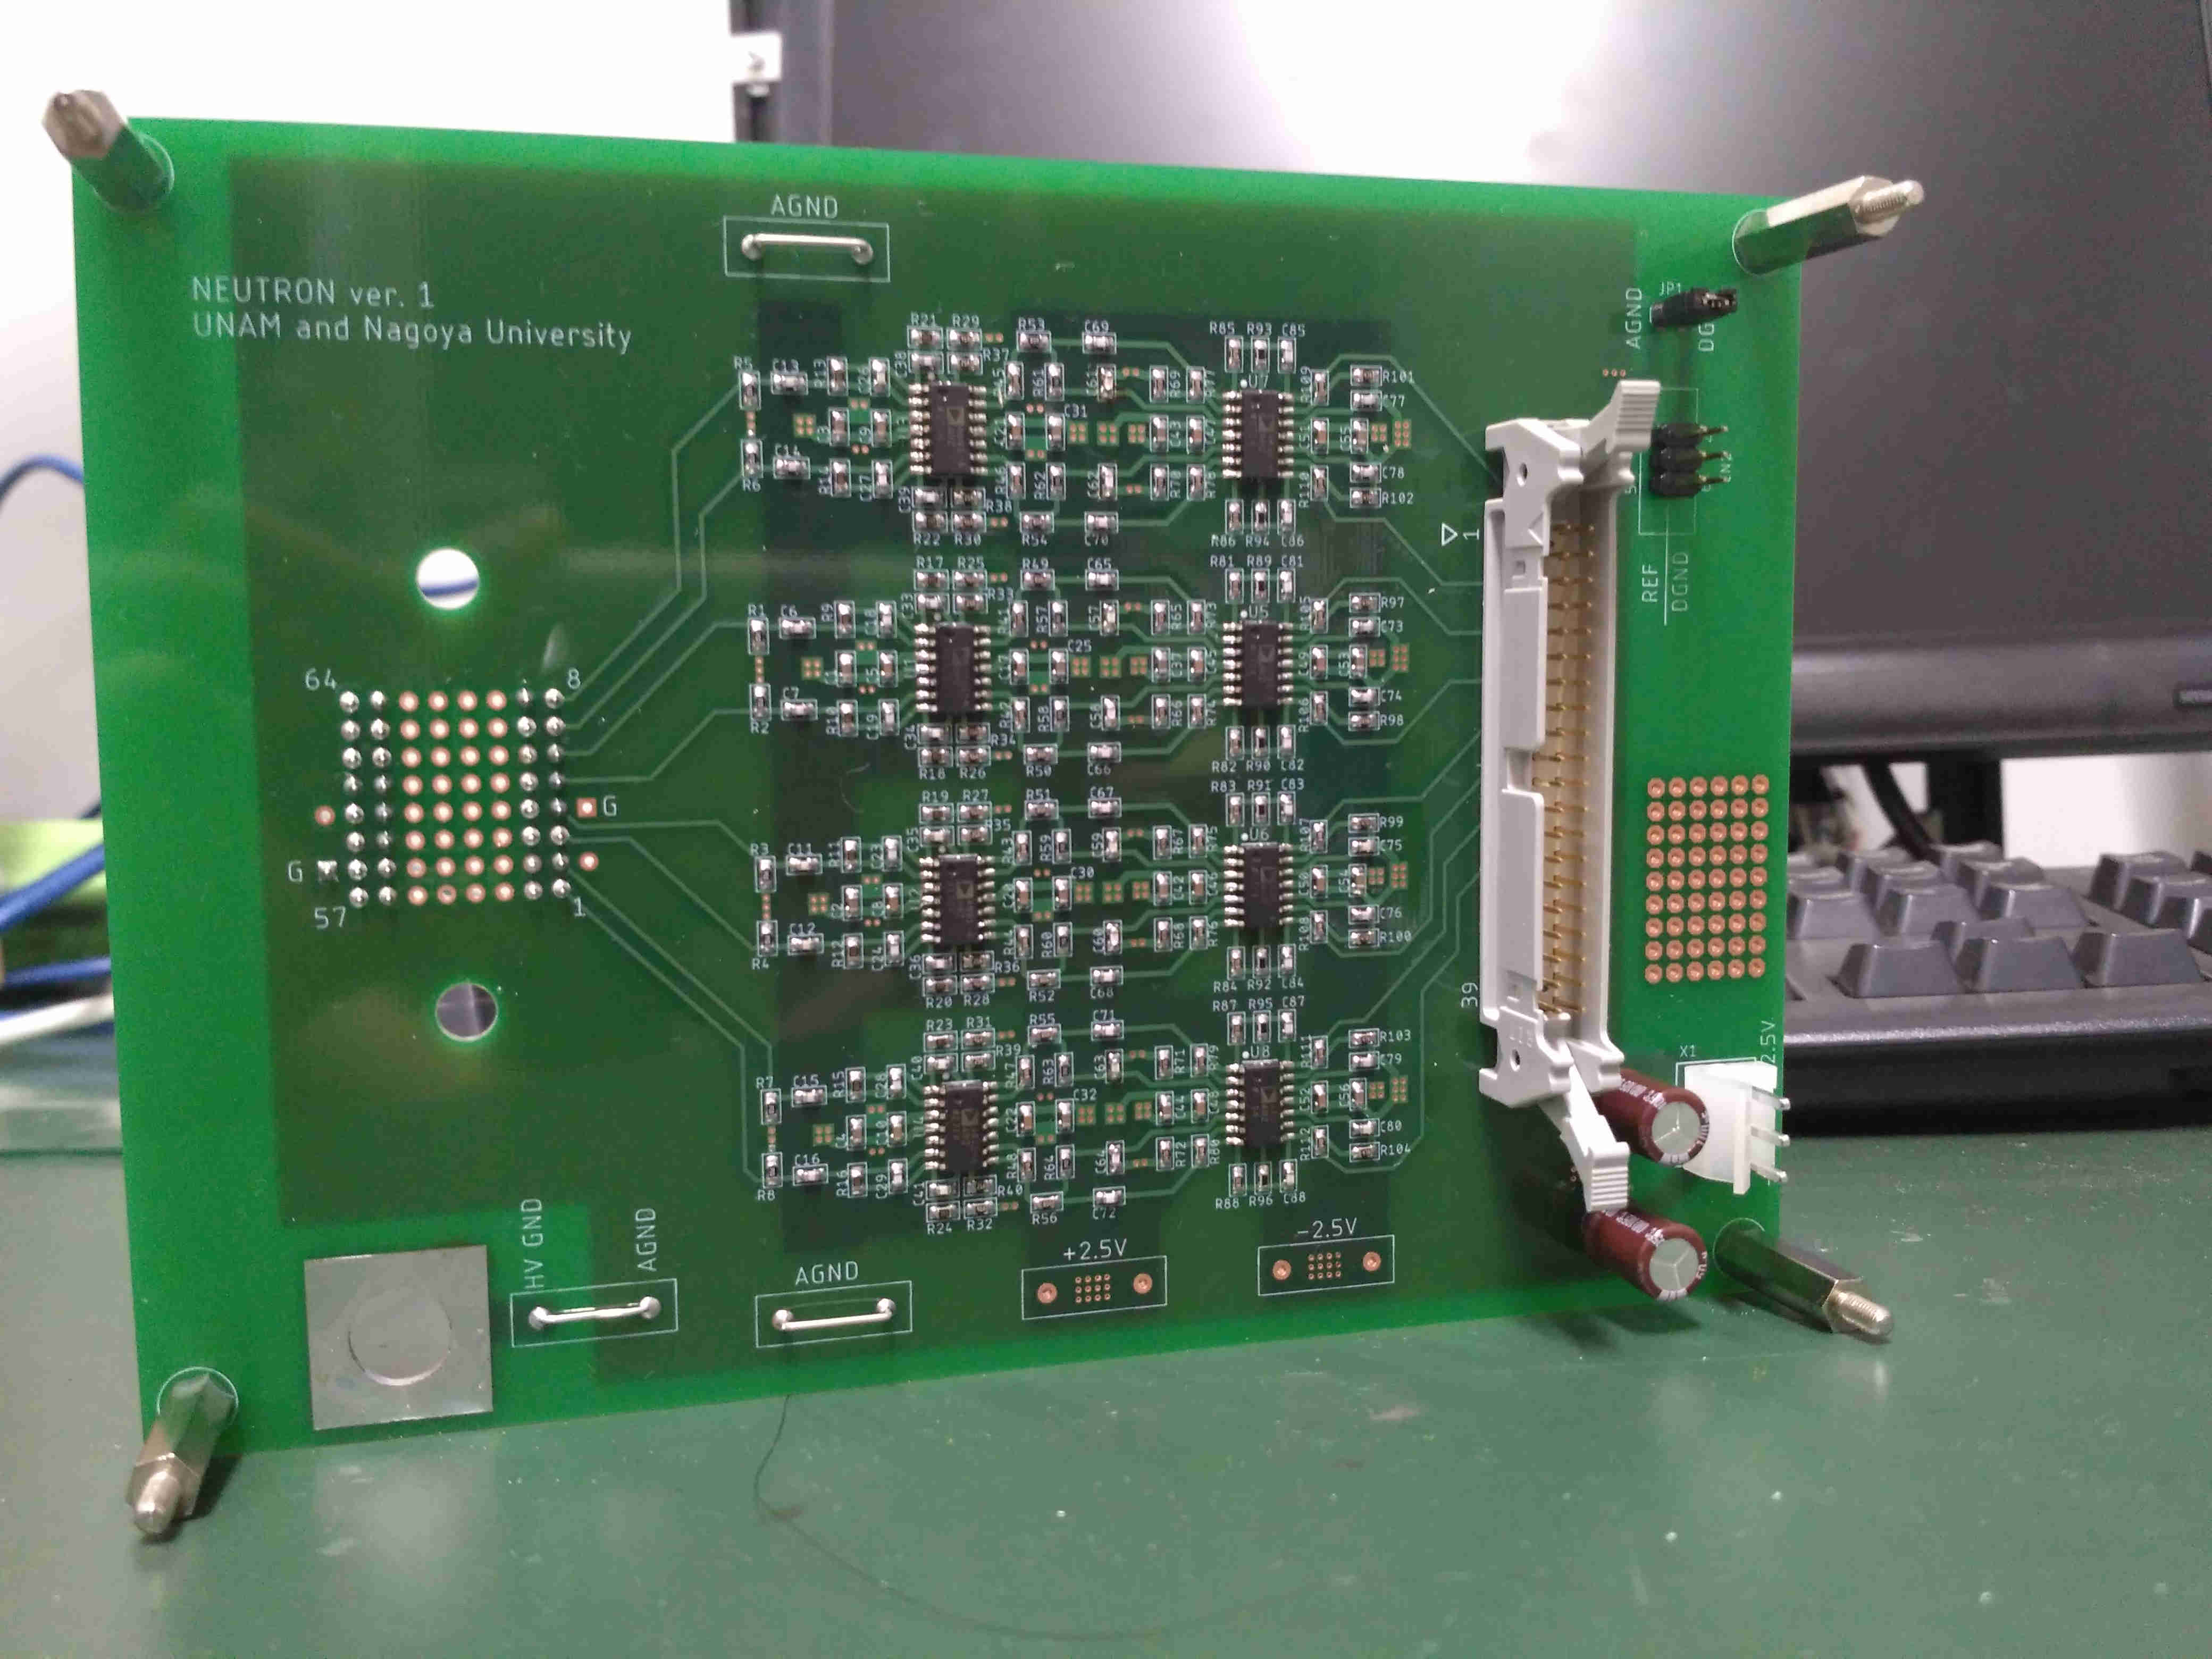
\includegraphics[width=\textwidth]{neutron_ver1.jpg}
	\caption{Tarjeta diseñada.}
	\label{fig:neutron-pcb}
  \end{subfigure}
  \begin{subfigure}[b]{0.49\textwidth}
	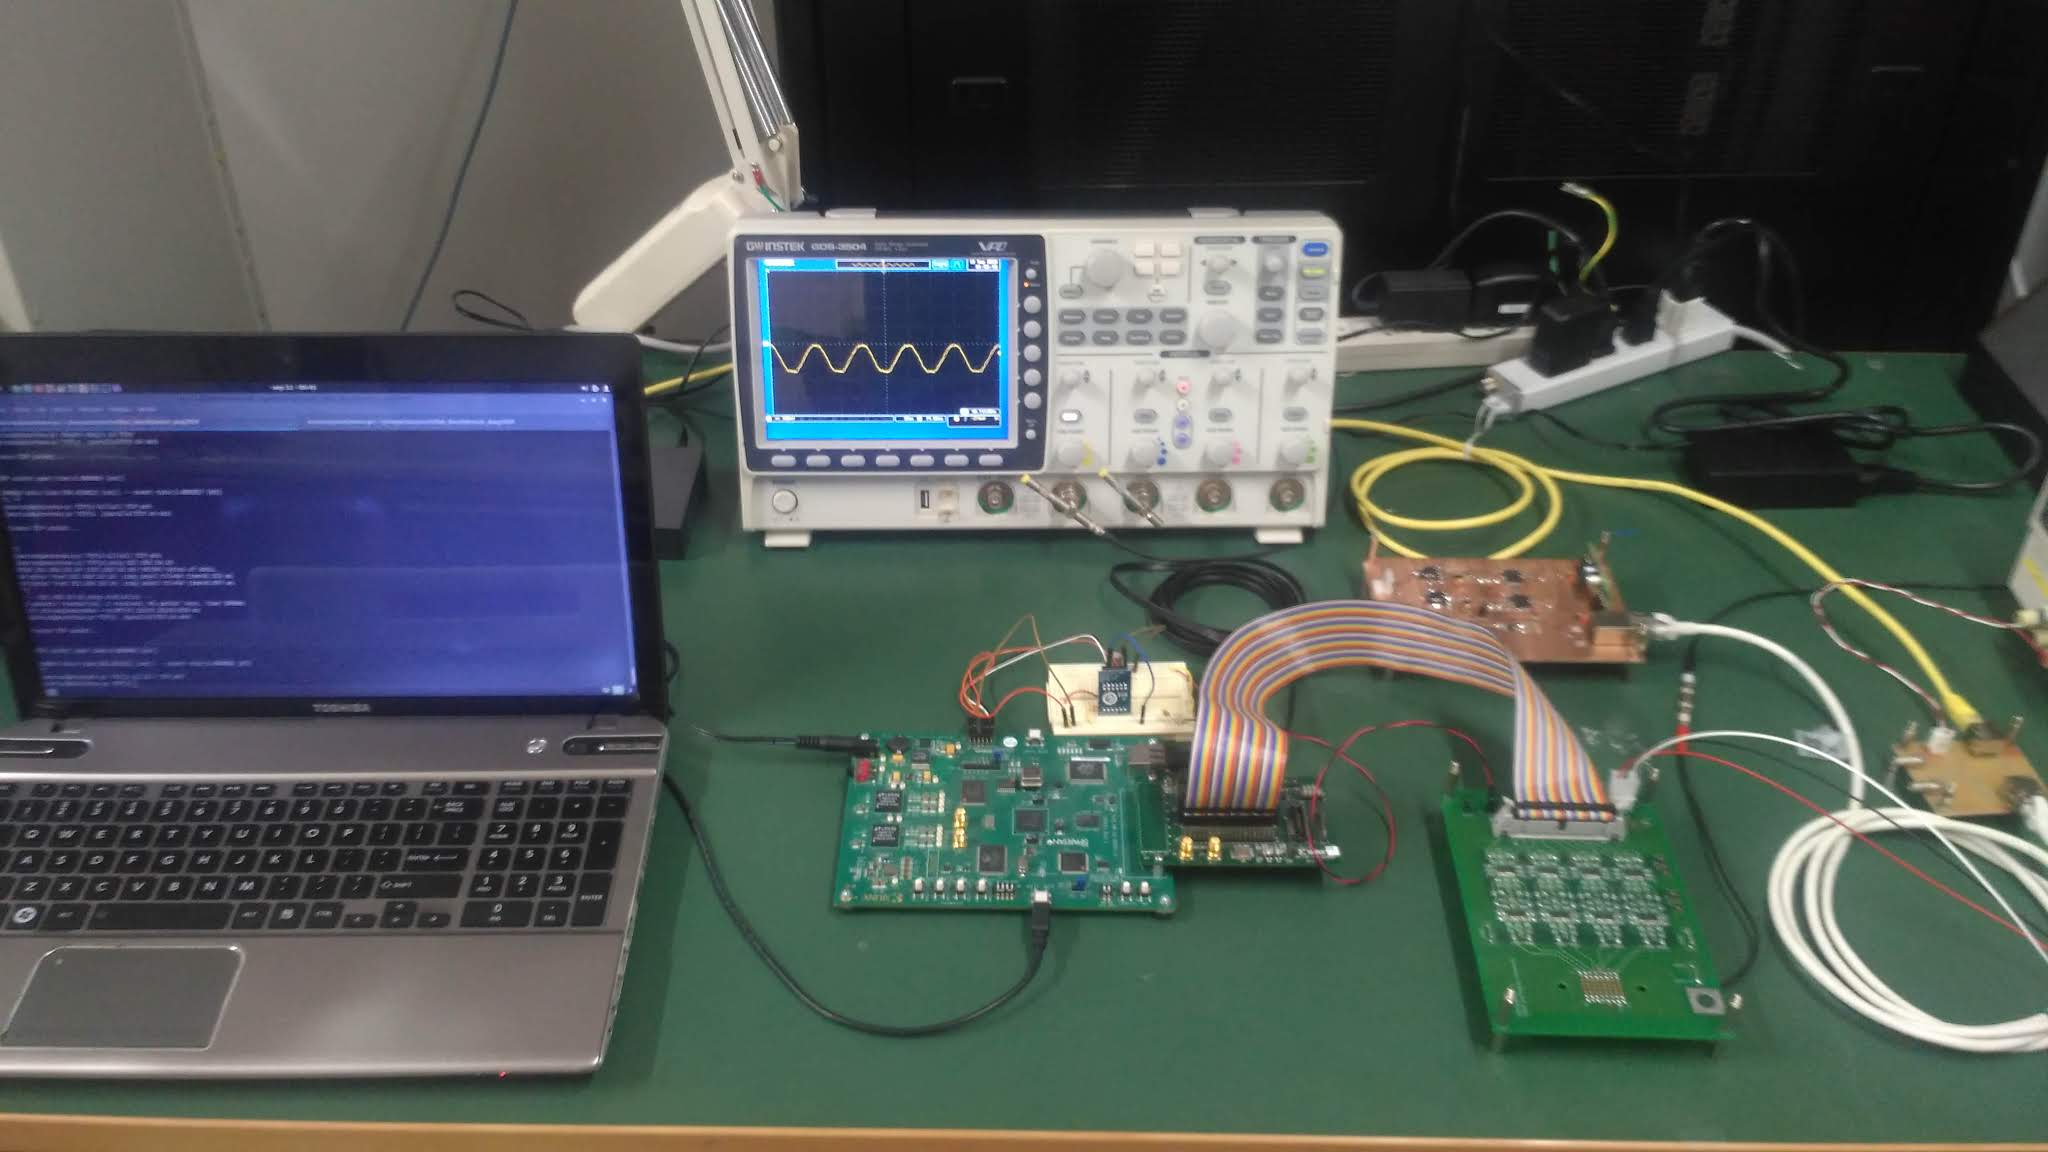
\includegraphics[width=\textwidth]{complete-system.jpg}
	\caption{Sistema en pruebas}
	\label{fig:complete-sys}
  \end{subfigure}
  \caption{Prototipo de la nueva electrónica del SciCRT desarrollado en la Universidad de Nagoya durante le verano de \num{2018}.}
  \label{fig:new-electronics}
\end{figure}

El resultado de la prueba usando LED con una carga equivalente a \SI{10}{pe} se observa en la figura \ref{fig:tdc-simexp}. El lienzo grande de la figura muestra la distribución de valores de TOT resultado del experimento, mientras que el lienzo pequeño contiene el resultado de una simulación de la electrónica usando la carga definida. Las diferencias entre el experimento y la simulación se observan en los datos alrededor de \SI{5}{\ns} y en eventos mayores a \SI{80}{\ns}. Estos efectos son producidos por el ruido de electrónico (pedestal) y contaminación de fotones, respectivamente. Ambos procesos no están incluidos en el modelo de la simulación.

Las fluctuaciones periódicas que se observan en el distribución experimento (como por ejemplo alrededor de \SI{20}{\ns}) son producto del jitter en las señales de reloj y LED, además de otros efectos no lineales del TDC. Esta situación se describió previamente en este capitulo, y requiere de un estudio más profundo para determinar sus efectos en la pérdida de precisión del sistema. A pesar de estas discrepancias, las similitudes entre la simulación y el experimento validan nuestra metodología.

La versión final de la electrónica actualmente está en construcción y pronto comenzará a probarse en el sitio. Para esta versión usaremos el circuito ADA4807, ya que tiene excelentes características para operar en alta montaña. Usando este amplificador estimamos un consumo de potencia de \SI{700}{\mW}, lo cual es aproximadamente \num{5} mayor a la electrónica original diseñada usando ASICs. A pesar de esto, la integración de diversas funciones en un solo sistema gracias al uso del FPGA, nos proyecta un consumo total de potencia de \SI{5}{\W} por unidad, lo cual representa un \SI{50}{\percent} de ganancia en comparación por el sistema de adquisición de datos original.

\begin{figure}
        \centering
        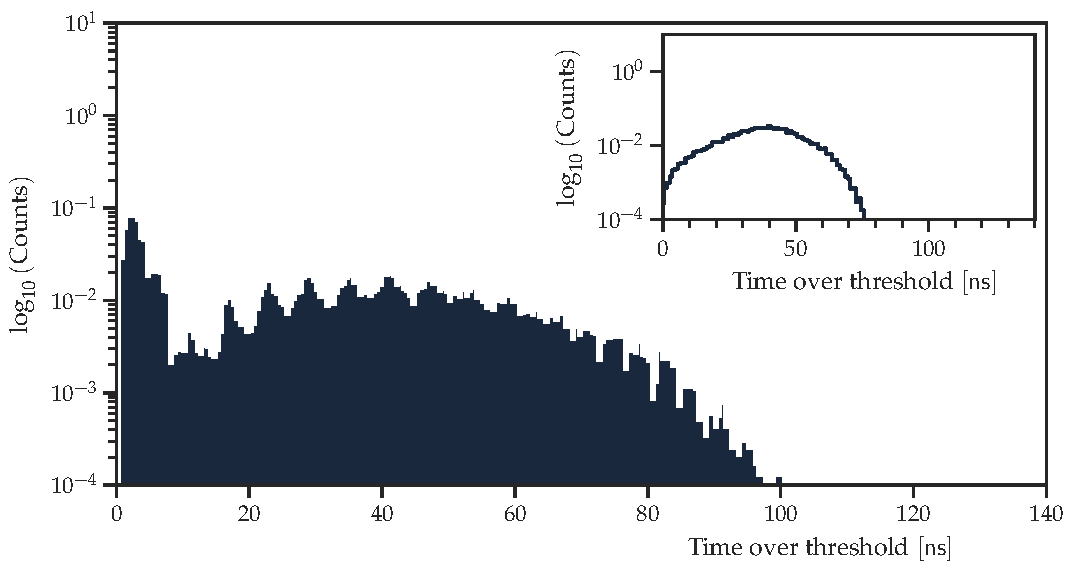
\includegraphics[width=\textwidth]{tdc_sim-exp.pdf}
        \caption{Distribución experimental de TOT (lienzo grande) y simulación (canvas pequeño) para una carga equivalente de \SI{10}{pe} utilizando un TDC de \SI{8}{\bit} con \SI{1}{\ns} resolution.}
        \label{fig:tdc-simexp}
\end{figure}
